 %%%%%%%%%%%%%%%%%%%%%%%%%%%%%%%%%%%%%%%%%%%%%%%%%%%%%%%%%%%%%%%%%%%%%%
% LaTeX Template: Newsletter  % Source: http://www.howtotex.com
%
% Feel free to distribute this example, but please keep the referral
% to howtotex.com
% Date: September 2011 
%%% ---------------
%%% PREAMBLE
%%% ---------------
\documentclass[10pt,a4paper]{article}

% Define geometry (without using the geometry package)
\setlength\topmargin{-48pt}
\setlength\headheight{13pt}
\setlength\headsep{25pt}
\setlength\marginparwidth{-20pt}
\setlength\textwidth{7.0in}
\setlength\textheight{9.5in}
\setlength\oddsidemargin{-30pt}
\setlength\evensidemargin{-30pt}

\frenchspacing						% better looking spacing

% Call packages we'll need
\usepackage[english]{babel}			% english
\usepackage{graphicx}				% images
\usepackage{amssymb,amsmath}		% math
\usepackage{multicol}				% three-column layout
\usepackage{url}					% clickable links
\usepackage{marvosym}				% symbols
\usepackage{wrapfig}				% wrapping text around figures
\usepackage{arev} 
\usepackage[T1]{fontenc}			% https://tex.stackexchange.com/questions/59403/what-font-packages-are-installed-in-tex-live % font encoding https://latexref.xyz/fontenc-package.html
\usepackage{blindtext}				% dummy text
\usepackage{datetime}				% custom date
	\newdateformat{mydate}{\monthname[\THEMONTH] \THEYEAR}
\usepackage[pdfpagemode=FullScreen,
			colorlinks=false]{hyperref}	% links and pdf behaviour

% Customize (header and) footer
\usepackage{fancyhdr}
\pagestyle{fancy}
\lfoot{	\footnotesize 
		RITMO report, Bodies in Concert \\
		\Mundus\ \href{https://www.uio.no/ritmo/english/news-and-events/events/artistic-performances/2023/symphony-experiment/index.html}{Lydo Concerts 2023}	\quad										\quad
		\Letter\ \href{mailto:finn.upham@imv.uio.no}{finn.upham@imv.uio.no}
	  }
\cfoot{}
\rfoot{\footnotesize ~\\ Page \thepage}
\renewcommand{\headrulewidth}{0.1pt}	% no bar on top of page
\renewcommand{\footrulewidth}{0.4pt}	% bar on bottom of page

%%% ---------------
%%% DEFINITIONS
%%% ---------------

% Define separators
\newcommand{\HorRule}[1]{\noindent\rule{\linewidth}{#1}} % Creating a horizontal rule
\newcommand{\SepRule}{\noindent							 % Creating a separator
						\begin{center}
							\rule{250pt}{1pt}
						\end{center}
						}						

% Define Title en News input
\newcommand{\JournalName}[1]{%


		\begin{center}	
		\noindent\raisebox{\dimexpr2.1\baselineskip-\height}{
\includegraphics[height=0.5in]{RITMO-hovedmerke-290818_150px.png}}
			\Huge \usefont{T1}{pag}{m}{n}
			#1%
		\end{center}	
		\par \normalsize \normalfont}
		
\newcommand{\JournalIssue}[1]{%
		\hfill \textsc{\mydate \today}%, No #1}
		\par \normalsize \normalfont}

\newcommand{\NewsItem}[1]{%
		\usefont{T1}{pag}{b}{n} 	
		\large #1 \vspace{4pt}
		\par \normalsize \normalfont}
		
\newcommand{\NewsAuthor}[1]{%
			\hfill by \textsc{#1} \vspace{4pt}
			\par \normalfont}		

%%% ---------------
%%% BEGIN DOCUMENT
%%% ---------------
\begin{document}
% Title	
% -----
\JournalIssue{1}
\JournalName{Bodies in Concert: Performer summary}
\noindent\HorRule{3pt} \\[-0.75\baselineskip]
\HorRule{1pt}
% -----

% Front article
% -----
\vspace{0.5cm}
	\SepRule
\vspace{0.5cm}

\begin{center}
\begin{minipage}[h]{0.75\linewidth}
	\begin{wrapfigure}{l}{0.41\textwidth}
		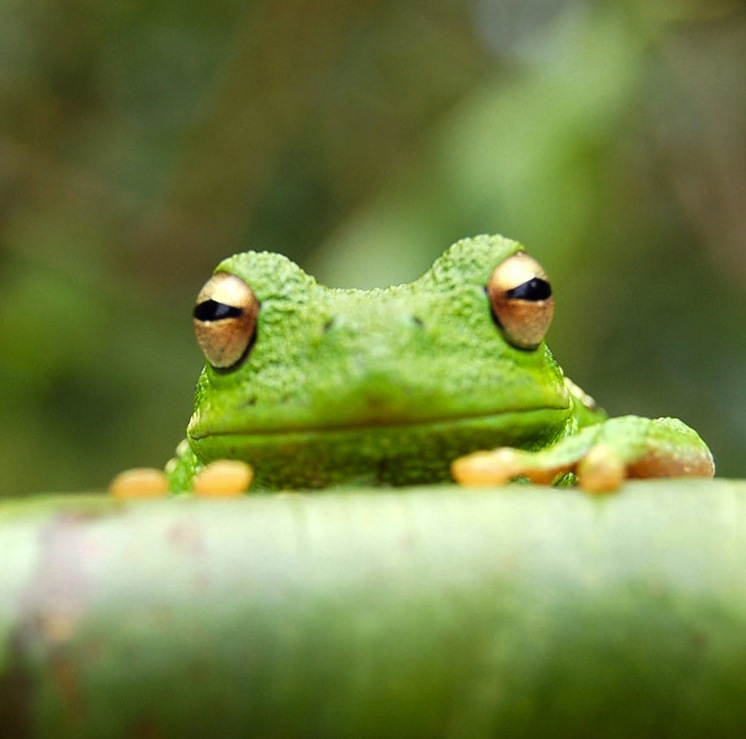
\includegraphics[width=0.42\textwidth]{frog.jpg}
		\\	% this spacer is needed to make the text on the right fit OK
	\end{wrapfigure}
	
	\NewsItem{Frog eats monkey}
	\emph{\blindtext}
\end{minipage}
\end{center}
% -----


% Other news (1)
% -----
\vspace{0.5cm}
	\SepRule
\vspace{0.5cm}
\begin{multicols}{3}
	\NewsItem{Monkey eats elephant}
	\NewsAuthor{F. Wenneker}
	\blindtext[2] 
% -----

\vspace{1cm}
% Other news (2)
% -----
\NewsItem{Elephant eats frog}
\NewsAuthor{J. Doe}
	\blindtext[1]
		\begin{center}
			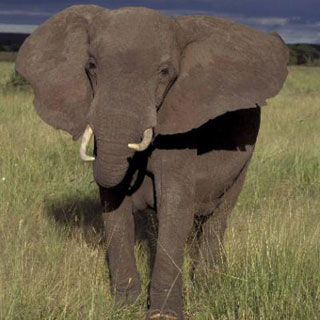
\includegraphics[width=0.8\linewidth]{elephant}
		\end{center}
		\blindtext[1]
\end{multicols}

\section{Trumpet}
 
This document shares some outputs from data collected with the equivitals.
\begin{figure}
\includegraphics[width=\linewidth]{/Users/finn/Desktop/Current_Projects/Stavanger/Summaries/Plots/Waves/Resp_BR602_Tcha_waves.jpg}
\caption{Respiration during each performance of one piece.}
\label{6Resp}
\end{figure}
\end{document}

% -----
\end{document} 
